% ------------------------------------------------------------%
% 2020-12-05
% 2015-2020 - Emerson Ribeiro de Mello - mello@ifsc.edu.br
% ------------------------------------------------------------%
\documentclass[11pt]{classes/ifscarticle}
\usepackage{classes/ifscutils}
\usepackage[alf]{abntex2cite} % Citações padrão ABNT

\renewcommand*{\theusecase}{UC-\thesection.\arabic{usecase}}


\usepackage{lipsum}

\AtBeginDocument{\thispagestyle{empty}}
\begin{document}
% ------------------------------------------------------------%
% Capa
% ------------------------------------------------------------%
\begin{center}

% Logotipo do órgão

\includegraphics[scale=.7]{classes/imagens/ifsc-v}
\vspace{7.5cm}

% Título
{\huge \bfseries Relatório Sistemas de Comunicação 1}

\vspace{.5cm}

% Subtítulo
{\large \bfseries  Laboratório - Sinais de Espectro}

\vfill
\end{center}

% Autor(es)
{\noindent \large \bfseries 
Sarom Torres%
%\\[.5em] Segundo Autor do Trabalho%
}

% Data que o relatório foi gerado
\begin{flushright}
08 de dezembro de 2020
\end{flushright}

\clearpage
\pagestyle{firstpage}
% ------------------------------------------------------------%

% ------------------------------------------------------------%
% Adicionando sumário
% ------------------------------------------------------------%
\tableofcontents
\clearpage

% ------------------------------------------------------------%
% Início do documento
% ------------------------------------------------------------%

\section{Introdução}
\label{cap:introducao}

O presente relatório tem por objetivo detalhar as atividades de laboratório referentes à revisão de Sinais de Espectros da disciplina de Sistemas de Comunicação 1. Tais atividades visam o fortalecimento dos conceitos de sinais no domínio do tempo e no domínio da frequência, tais como: energia e potência de um sinal, transformada de Fourier, autocorrelação, ruido branco, filtros, entre outros.

Para tanto, foram desenvolvidas três atividades. A primeira atividade (A1) consiste na simulação da soma três sinais senos com diferentes amplitudes e frequências a fim de observar suas características no domínio do tempo e da frequência. Além disso, nessa atividade são analisados dados de potência média do sinal e densidade espectral do sinal.

Na segunda atividade (A2) três sinais e três filtros com diferentes características foram desenvolvidos a fim de observar o comportamento do sinal, no domínio do tempo e da frequência, após a sua passagem por esses filtros .

Na terceira atividade (A3) foram simulados um sinal aleatório gaussiano e um filtro a fim de compreender os conceitos de autocorrelação e ruído branco.

Para as simulações realizadas foi utilizado o software Matlab. Nos conceitos teóricos são apresentados breves resumos sobre a base teórica necessária no desenvolvimento das atividades, nas Atividades são descritas das atividades desenvolvidas e debatidos os resultados obtidos. 


\section{Conceitos Teóricos}
\label{sec:conceitos}

Os sinais de espectro podem ser analisados através de diversas características, tais como sua energia, potência média, sua transformada de Fourier, sua autocorrelação, entre outros. Abaixo segue a descrição de alguns elementos utilizados para a análise dos sinais. 

\subsection{Energia e Potência Média de um Sinal}
\label{sec:potencia}
Em algumas aplicações, o sinal analisado está relacionado com a quantia de energia e potência que um sistema pode capturar. Classificar um determinado sinal como sinal de energia ou de potência facilita seu tratamento matemático.

Para ser considerado um sinal de energia, a energia dissipada de um sinal deve ser avaliada dentro de um intervalo de tempo e deve ser finita e sua potência média deve ser zero. 

A potência média de um sinal é compreendida como a taxa pela qual a energia é entregue, sendo que para ser considerado um sinal de potência, a potência dele deve ser finita e sua energia deve ser infinita.

O cálculo da potência média dissipada pode ser feito através da \autoref{eq:pot}.

 \begin{equation}
     P_x^T = \frac{1}{T}\int_{-T/2}^{T/2} x^2(t) dt
     \label{eq:pot}
 \end{equation}


Geralmente sinais aleatório e sinais periódicos são classificados como sinais de potência.



\subsection{Densidade Espectral de Potência}
\label{sec:DEP}

A densidade espectral de um sinal está relacionado com a distribuição de sua energia (DEE) ou potência (DEP) no domínio da frequência. Isto significa dizer que é possível avaliar em quais frequências a energia ou potência de um sinal está concentrada.  


\subsection{Transformada de Fourier}
\label{sec:transformada}

A Transformada de Fourier permite a representação de um sinal no domínio do tempo em suas componentes de frequência.

\subsection{Autocorrelação}
\label{sec:autocorrelacao}

A autocorrelação refere-se a correspondência de um sinal com sua cópia deslocada.

\subsection{Filtros Ideais}
\label{sec:filtros}

Os filtros, geralmente, são utilizados para a separação de um sinal de outras componentes indesejadas, tais como ruídos, interferências, etc.
Um filtro ideal é aquele que recupera as características do sinal sem distorção alguma. 

Os filtros podem ser categorizados de diversas formas, por exemplo:
um filtro passa-baixa recupera apenas frequências abaixo da frequência de corte, um filtro passa-faixa recupera o sinal dentro de uma determinada faixa de corte, um filtro passa-alta recupera apenas frequências acima da frequência de corte.

\subsection{Ruído Branco}
\label{sec:ruido}

O ruído branco também é conhecido como ruído térmico, pois é originado pela agitação dos elementos dissipativos do circuito. O ruído branco é constante para todas as frequências, sendo assim a densidade espectral dele depende da banda e não da frequência que o sistema está operando. 

A autocorrelação do ruído branco é um impulso, o que significa dizer que uma amostra de ruído é completamento descorrelacionada de outra.

\section{Atividades}
\label{sec:atividades}


%------------------------------|
%       Atividade 1            |
%------------------------------|

\subsection{Atividade 1}
\label{sec:A1}

A primeira simulação consiste em gerar um sinal composto pela somatória de três sinais senos com diferentes amplitudes e frequências.
O objetivo é analisar esses sinais no domínio do tempo e da frequência, além de encontrar sua potência média e sua densidade espectral. 

\subsubsection{Sinais no domínio do tempo}
Na \autoref{eq:y1}, \autoref{eq:y2}, \autoref{eq:y3} e \autoref{eq:s_t} estão descritos os sinais simulados.


 \begin{equation}
    y_1(t) = 6 \sin (2\pi\times10^3t)
     \label{eq:y1}
 \end{equation}

 \begin{equation}
    y_2(t) = 2 \sin (2\pi\times3\times10^3t)
     \label{eq:y2}
 \end{equation}
 
  \begin{equation}
    y_3(t) = 4 \sin (2\pi\times5\times10^3t)
     \label{eq:y3}
 \end{equation}
 
  \begin{equation}
     s(t) = y_1(t) + y_2(t) + y_3(t)
     \label{eq:s_t}
 \end{equation}


\begin{figure}[ht]
    \centering
    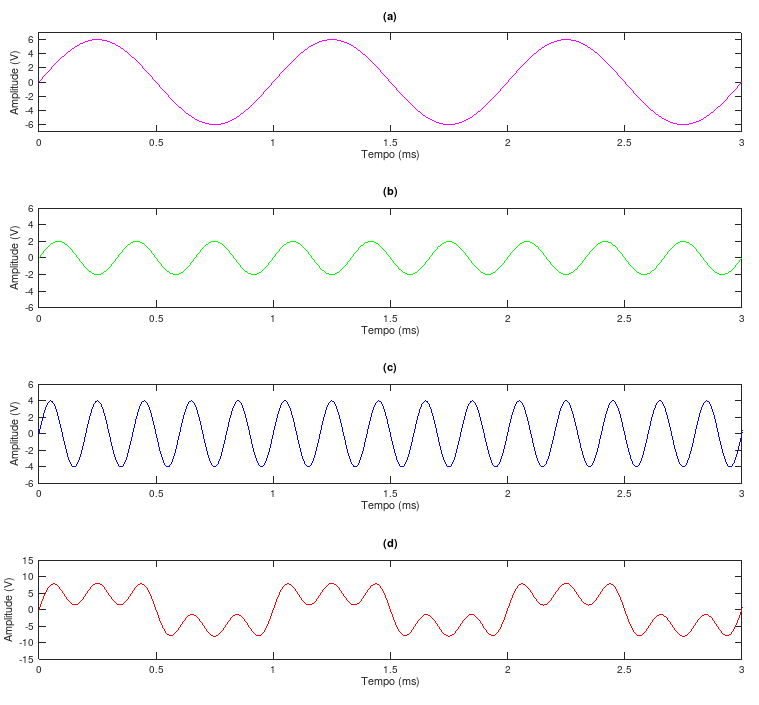
\includegraphics[width=.6\linewidth]{figuras/q1_sen_t.png}
    \caption{\textbf{(a)} - $y_1(t)$, \textbf{(b)}  - $y_2(t)$, \textbf{(c)}  -$y_3(t)$, \textbf{(d)} - s(t). Fonte Própria. }
    \label{fig:q1_sen_t}
\end{figure}

 Na \autoref{fig:q1_sen_t}-a o sinal tem amplitude de 6V e frequência de 1kHz, na \autoref{fig:q1_sen_t}-b a amplitude é de 2V e frequência de 3KHz, na \autoref{fig:q1_sen_t}-c a amplitude é de 4V e frequência de 5KHz. Como os três sinais possuem frequências diferentes ao serem somados suas amplitudes também se somam gerando como resultado a onda da \autoref{fig:q1_sen_t}-d. 

Vale salientar que, como os períodos desses sinais são diferentes e em nenhum momento os picos ou vales ocorrem no mesmo instante de tempo a amplitude do sinal s(t) nunca chega à soma das três amplitudes.
Caso o sinal s(t) recebesse o somatório de mais sinais senos com maiores frequências ele tenderia a se tornar um onda quadrada.

\subsubsection{Sinais no domínio da frequência}

Para a análise dos sinais no domínio da frequência foi utilizada a função \texttt{fft} do Matlab que faz a transformada rápida de Fourier do sinal. Conforme abordado na \autoref{sec:transformada} é através de transformada de Fourier que obtemos as componentes de frequência dos sinais.
Na \autoref{fig:q1_sen_f} estão representadas as transformadas de Fourier de cada um deles.

\begin{figure}[ht]
    \centering
    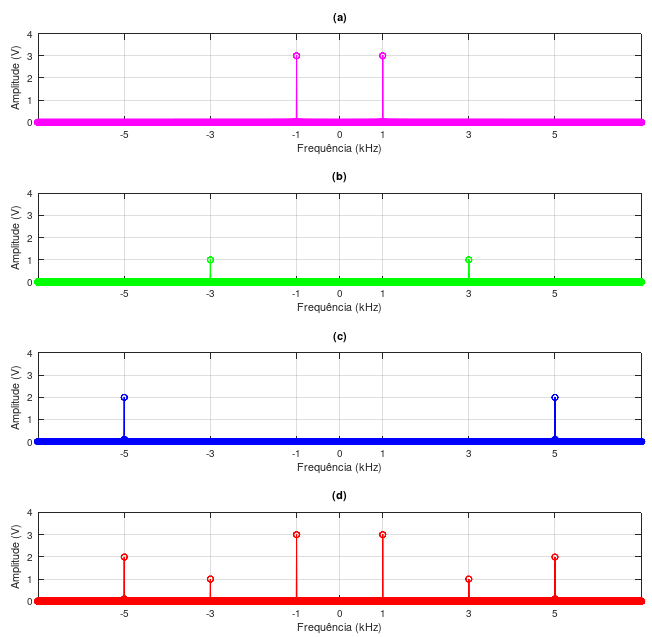
\includegraphics[width=.6\linewidth]{figuras/q1_sen_f.png}
    \caption{\textbf{(a)} - Y1(f), \textbf{(b)}  - Y2(f), \textbf{(c)}  - Y3(f), \textbf{(d)} - S(f). Fonte Própria. }
    \label{fig:q1_sen_f}
\end{figure}

 É possível notar que a transformada do seno é o impulso deslocado para a frequência no qual o sinal opera. Devido o seno também ser representado conforme a \autoref{eq:sen} ao realizar a transformada a amplitude cai pela metade, sendo que nas representações (a), (b) e (c) da \autoref{fig:q1_sen_f} a amplitude é de 3V, 1V e 2V respectivamente.
 
 \begin{equation}
     \sin \theta = \frac{(e^{j\theta} - e^{-j\theta})}{2j}
     \label{eq:sen}
 \end{equation}

Ao fazer a transformada do sinal aparece um impulso na frequência negativa de igual valor. Isso se dá ao fato de o círculo trigonométrico, no qual são representados os números complexos da \autoref{eq:sen}, poder tanto ser compreendido no sentido anti-horário (frequências positivas) como no sentido horário (frequências negativas).

Além disso, o espectro da \autoref{fig:q1_sen_f}-d mostra as três frequências existentes no sinal s(t) que são oriundas dos sinais que compões o somatório (\autoref{eq:y1}, \autoref{eq:y2}, \autoref{eq:y3}).

\newpage
\subsubsection{Potência média}

Para descobrir potência média do sinal s(t) foi utilizada a \autoref{eq:pot}. Portanto, na simulação foi usada a função \texttt{norm} do Matlab, a qual faz o cálculo do módulo de um vetor, seu resultado foi elevado ao quadrado e divido pelo tamanho do vetor. Dessa foma, se obteve o valor de 28 \textit{Watts} de potência média do sinal.

Vale salientar, que o cálculo da potência média de s(t) é mais adequado, visto que ele é um sinal periódico e portanto, considerado um sinal de potência e não de energia.

\subsubsection{Densidade Espectral de Potência}

Para calcular a densidade espectral de potência foi utilizada a função \texttt{pwelch} do Matlab. Essa função calcula a DEP de um sinal baseado na taxa de amostragem.

\begin{figure}[ht]
    \centering
    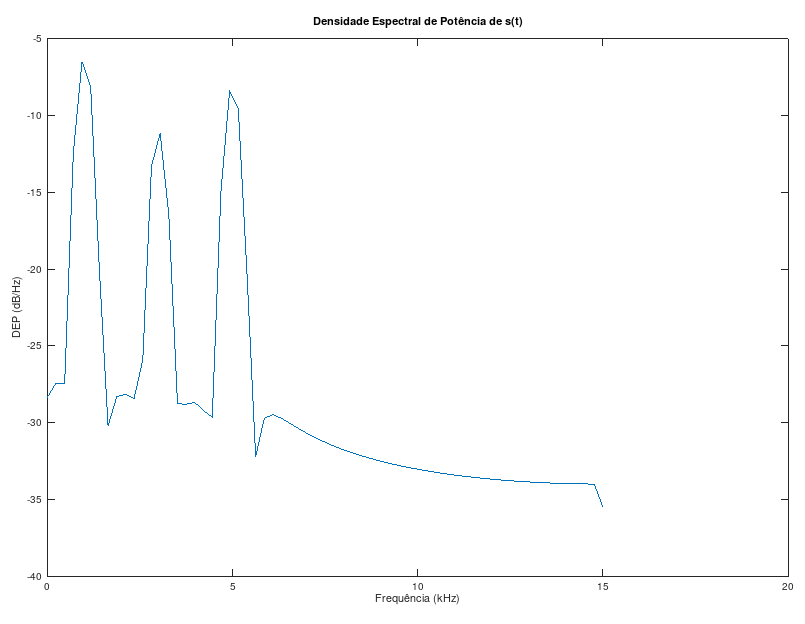
\includegraphics[width=.6\linewidth]{figuras/q1_dep.png}
    \caption{Densidade Espectral de Potência do sinal s(t) com 30 amostras. Fonte Própria.}
    \label{fig:q1_dep}
\end{figure}

A \autoref{fig:q1_dep} mostra a DEP do sinal s(t) com 30 amostras. Pode-se observar que a potência do sinal está concentrada nas frequências de 1kHz, 3kHz e 5kHz, sendo que há pouca energia nas demais frequências. 

\newpage
%------------------------------|
%       Atividade 2            |
%------------------------------|
\subsection{Atividade 2}
\label{sec:A2}

\subsubsection{Sinais no domínio do tempo}

Na atividade 2 foram simulados 3 senoides com diferentes amplitudes e frequências, um sinal composto pela somatória desses três sinais e 3 filtros ideais com diferentes frequências de corte. O objetivo deste experimento é analisar o comportamento desses sinais no domínio do tempo e da frequência após sua passagem por diferentes filtros.

O sinais realizados estão especificados nas equações abaixo e seu comportamento possui as mesmas características que os sinais criados da \autoref{sec:A1}, sendo que se diferenciam apenas na amplitude.

 \begin{equation}
     y_1(t) = 5 \sin (2\pi\times10^3t)
     \label{eq:q2_y1}
 \end{equation}

 \begin{equation}
     y_2(t) = \frac{5}{3} \sin (2\pi\times3\times10^3t)
     \label{eq:q2_y2}
 \end{equation}
 
  \begin{equation}
     y_3(t) = 1 \sin (2\pi\times5\times10^3t)
     \label{eq:q2_y3}
 \end{equation}
 
  \begin{equation}
     s(t) = y_1(t) + y_2(t) + y_3(t)
     \label{eq:q2_s_t}
 \end{equation}

\subsubsection{Sinais no domínio da frequência}
Na \autoref{fig:q2_sen_f_t} estão os sinais criados e seu espectro de frequências obtido através da Transformada de Fourier.

\begin{figure}[ht]
    \centering
    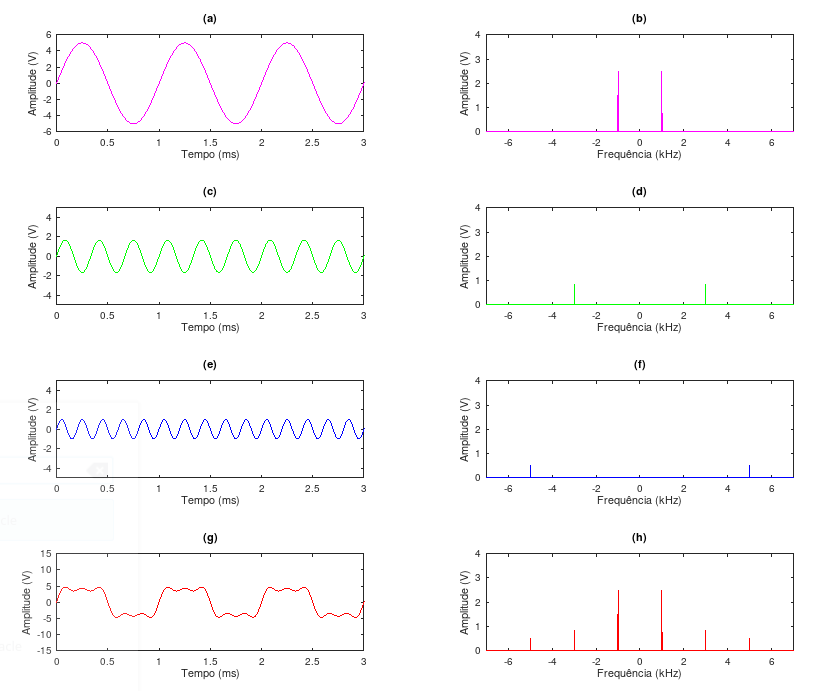
\includegraphics[width=.8\linewidth]{figuras/q2.sen_t_f.png}
    \caption{Sinais no domínio do tempo e da frequência. \textbf{(a)} - $y_1$(t),\textbf{(b)} - $Y_1$(f), \textbf{(c)}  - $y_2$(t), \textbf{(d)}  - $Y_2$(f), \textbf{(e)}  - $y_3$(t),  \textbf{(f)}  - $Y_3$(f), \textbf{(g)} - s(t), \textbf{(h)} - S(f) . Fonte Própria.}
    \label{fig:q2_sen_f_t}
\end{figure}

\subsubsection{Filtros}
Foram criados três filtros com a função \texttt{freqz} do Matlab. Um filtro passa-baixa com frequência de corte de 2kHz (\autoref{fig:ft_pb}), um filtro passa-alta de 4kHz (\autoref{fig:ft_pa}) e um filtro passa-faixa entre 2kHz e 4kHz (\autoref{fig:ft_pf}).

\begin{figure}[ht]
    \centering
    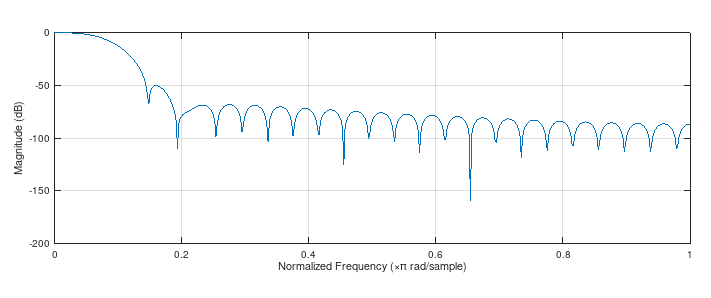
\includegraphics[width=.6\linewidth]{figuras/ft_pb.png}
    \caption{Filtro passa-baixa com frequência de corte de 2kHz. Fonte Própria.}
    \label{fig:ft_pb}
\end{figure}

\begin{figure}[ht]
    \centering
    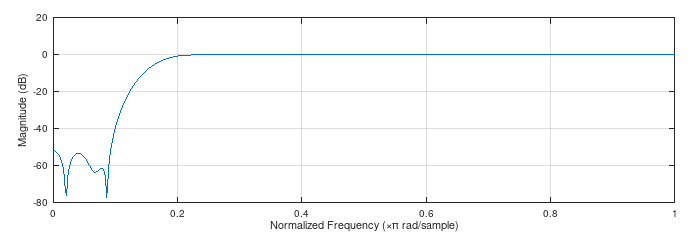
\includegraphics[width=.6\linewidth]{figuras/ft_pa.png}
    \caption{Filtro passa-alta de 4kHz. Fonte Própria.}
    \label{fig:ft_pa}
\end{figure}

\begin{figure}[ht]
    \centering
    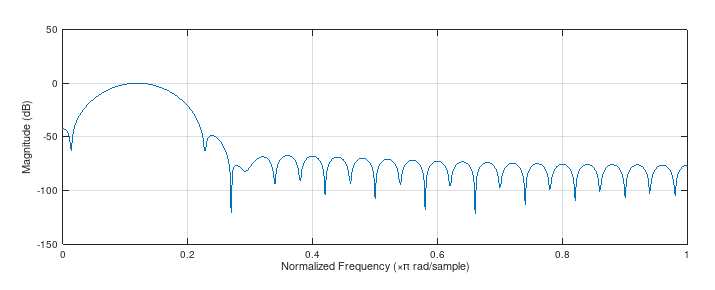
\includegraphics[width=.6\linewidth]{figuras/ft_pf.png}
    \caption{Filtro passa-faixa entre 2kHz e 4kHz. Fonte Própria.}
    \label{fig:ft_pf}
\end{figure}

Após a criação do filtros o sinal s(t) da \autoref{eq:q2_s_t} foi passado pelos filtros obtendo os resultados demonstrados na \autoref{fig:sinais_filt}.  

\begin{figure}[ht]
    \centering
    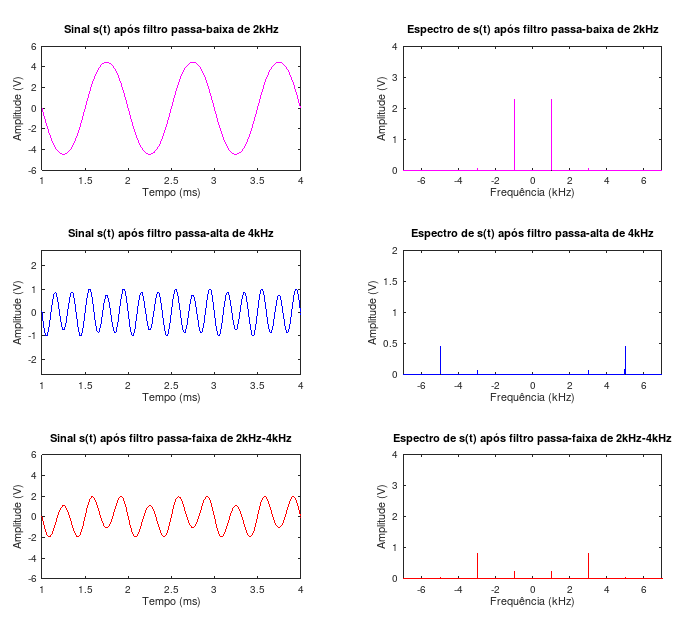
\includegraphics[width=.6\linewidth]{figuras/ft_sen_FT.png}
    \caption{Sinais filtrados representados no domínio do tempo e da frequência. Fonte Própria.}
    \label{fig:sinais_filt}
\end{figure}

\newpage
Como é possível observar na \autoref{fig:sinais_filt} quando o sinal foi filtrado para frequências menores que 2KHz resultou na sua componente senoidal de 1KHz, o mesmo ocorreu para o filtro passa-alta que permitiu a passagem apenas da componente de 5kHz e para o filtro passa-faixa a qual permitiu a passagem da componente de 3kHz.

\newpage

%------------------------------|
%       Atividade 3            |
%------------------------------|

\subsection{Atividade 3}
\label{sec:A3}

Neste exercício foi gerado um vetor gaussiano (\autoref{fig:dist_gau}) para representar um sinal de ruído branco de duração de 1 segundo. A amostragem utilizada a fim de gerar 1 segundo de ruído branco foi de 10kHz.
Além disso foi gerado um filtro com frequência de corte de 10 kHz para fazer a filtragem do ruido.
É possível observar o ruido plotado no domínio do tempo(\autoref{fig:ruido_te}). 

\begin{figure}[ht]
    \centering
    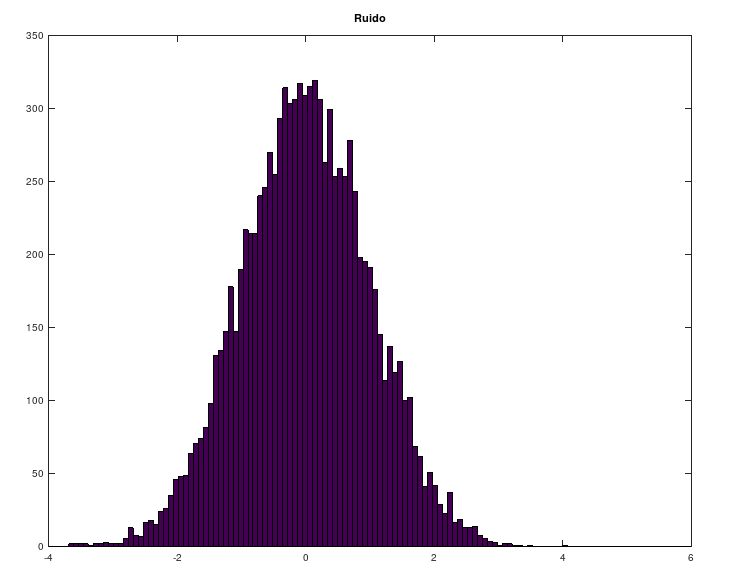
\includegraphics[width=.6\linewidth]{figuras/ruido_gau.png}
    \caption{Ruido com distribuição gaussiana. Fonte Própria.}
    \label{fig:dist_gau}
\end{figure}

\begin{figure}[ht]
    \centering
    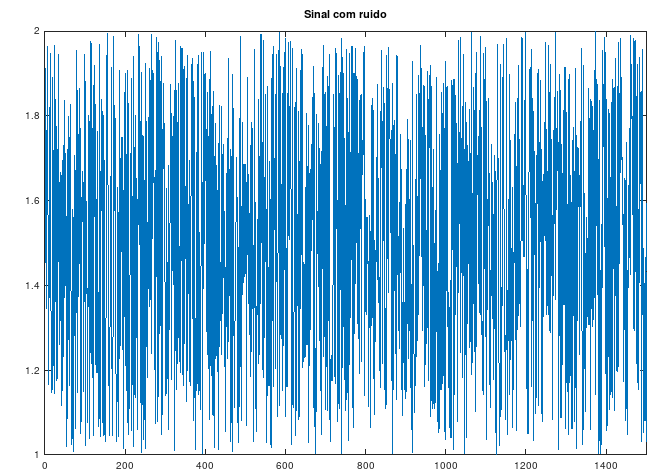
\includegraphics[width=.6\linewidth]{figuras/ruido_tempo.png}
    \caption{Ruido representado no domínio do tempo. Fonte Própria.}
    \label{fig:ruido_te}
\end{figure}

A \autoref{fig:autoruido_te} apresenta a autocorrelação do sinal ruído no qual é um impulso, visto que nenhuma amostra está correlacionada com a outra.

\begin{figure}[ht]
    \centering
    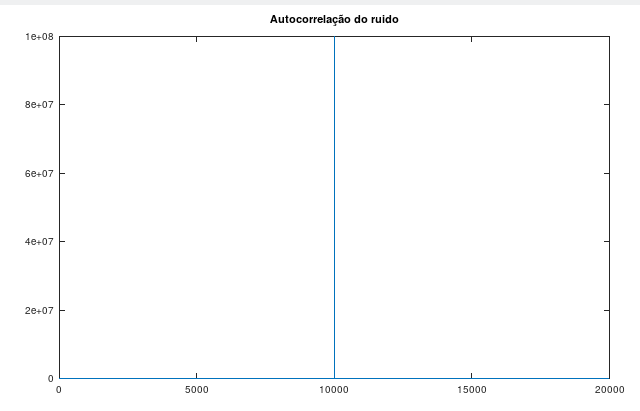
\includegraphics[width=.6\linewidth]{figuras/autoco.png}
    \caption{Autocorrelação do ruído. Fonte Própria.}
    \label{fig:autoruido_te}
\end{figure}

\newpage

Após a passagem pelo filtro o sinal apresenta o comportamento da \autoref{fig:ruido_fil} e é possível observar o histograma e ver que permanece com uma distribuição gaussiana

\newpage
\begin{figure}[ht]
    \centering
    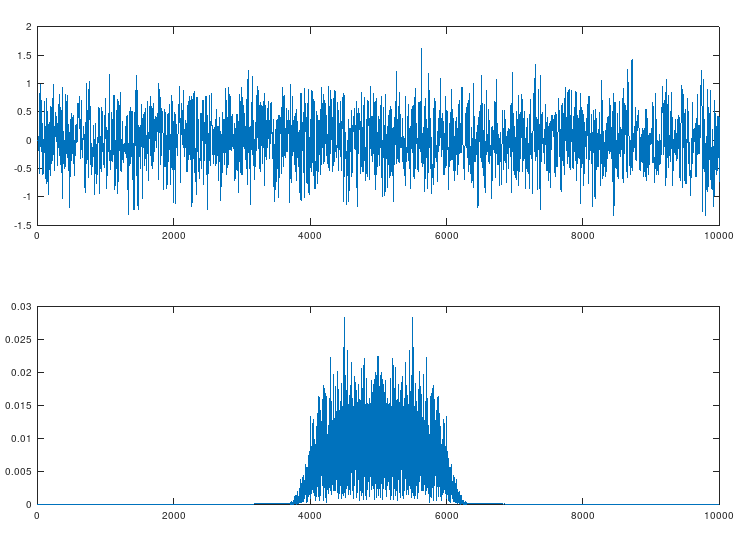
\includegraphics[width=.6\linewidth]{figuras/ruido_filtro.png}
    \caption{Ruido após passar pelo filtro. Fonte Própria.}
    \label{fig:ruido_fil}
\end{figure}

\begin{figure}[ht]
    \centering
    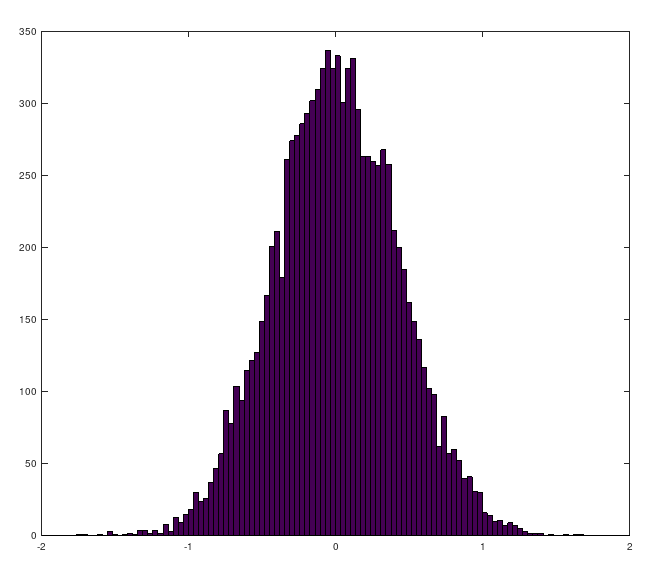
\includegraphics[width=.6\linewidth]{figuras/hist_ruido_filtrado.png}
    \caption{Histograma do ruído após passar pelo filtro. Fonte Própria.}
    \label{fig:hist_ruido}
\end{figure}

\newpage
\section{Conclusão}
\label{sec:conclusão}

Este trabalho apresentou os conceitos sobre sinais de espectros abordados em sala de aula. No \autoref{cap:introducao} foi apresentado o escopo geral do trabalho e seus principais objetivos. No \autoref{sec:conceitos} foram esclarecidos brevemente os principais tópicos utilizados para o desenvolvimento do laboratório e no \autoref{sec:atividades} foram descritas as atividades desenvolvidas e os resultados obtidos.

O presente trabalho fortaleceu os conhecimentos revisados na disciplina de Sistemas de Comunicação 1 assim como possibilitou a prática em software de simulação como o Matlab, sendo que a aplicação prática dos conceitos teóricos de Sinais de Espectro e o alcance de resultados permitiram sedimentar uma base de conhecimento para o restante da disciplina.


\section{Códigos desenvolvidos}
\label{sec:code_dev}

Segue o \href{https://github.com/sarom-torres/COM1/tree/master/AT-2020.2/Codigos_AE1}{link}
 para o acesso aos códigos.



% ----------------------------------------------------------
% Referências bibliográficas
% ----------------------------------------------------------
%\bibliography{referencias}
\end{document}


